\documentclass[9pt,twocolumn,twoside]{pnas-new}

\templatetype{pnasresearcharticle}

\title{Endosymbiotic fusion of elementary semi-organizations: a computable structural model of evolutionary complexification}

\author[a,1]{Tomas Veloz}

\affil[a]{Fundaci\'on para el Desarrollo Interdisciplinario de la Ciencia, la Tecnolog\'ia y las Artes, Santiago, Chile}

\leadauthor{Veloz}

\significancestatement{Endosymbiosis -- one organism engulfing another -- produced two of the largest jumps in the history of life: mitochondria and chloroplasts. We show that a purely structural, steady-state theory of metabolic networks (Chemical Organization Theory) can already detect the computational signature of that jump, without simulating any dynamics. Merging a host and a symbiont's metabolism through a handful of real transport reactions makes every single elementary semi-organization in the combined network draw on both partners -- a 100\% ``hybrid'' signature, reproduced on a hand-built toy model and on two independent real genome-scale reconstructions. The method also identifies, by simple knockout, which specific cross-fed metabolites are actually load-bearing for this integration -- a computable, falsifiable link between network structure and gene-retention patterns in reduced endosymbiont genomes.}

\authorcontributions{T.V. designed the study, wrote all code, ran all computations, and wrote the manuscript.}
\authordeclaration{The author declares no conflict of interest.}
\correspondingauthor{\textsuperscript{1}To whom correspondence should be addressed. E-mail: tveloz@gmail.com}

\keywords{chemical organization theory $|$ endosymbiosis $|$ metabolic networks $|$ elementary semi-organizations $|$ major evolutionary transitions}

\begin{abstract}
Chemical Organization Theory (COT) identifies the persistent, self-maintaining subnetworks of a reaction network -- its organizations -- from structure alone, without simulating dynamics. A companion result shows that supplying an \textit{Escherichia coli} genome-scale reconstruction with trace-metal cofactors does not add new elementary semi-organizations (ESOs); it \emph{fuses} existing ones into fewer, larger ones. Here we ask whether this fusion effect generalizes, and what happens when the ``inflow'' is not one abiotic species but an entire second living system's continuously regenerated output -- a structural description of endosymbiosis. We build a generic compartmentalized-union tool that merges a host and a symbiont network through an explicit, biologically justified interface, and a fusigenic-inflow search that ranks candidate inflows by how much they fuse rather than merely extend a network's ESO structure. On a hand-verified toy model and two independent real cases -- a mitochondrial-type merger self-derived from \textit{E. coli} core metabolism, and a chloroplast-type merger built from real, distinct genome-scale reconstructions of \textit{Saccharomyces cerevisiae} and \textit{Synechocystis} sp.\ PCC 6803 -- every single ESO of the merged network draws on machinery from both partners (100\% ``hybrid''), with mean ESO size growing 54--87\% beyond the better partner alone. Two distinct mechanisms produce this signature: capability-gain, where the food closure itself grows, and re-integration, where the same reachable chemistry reorganizes into fewer, larger modules. Verifying self-maintenance of every ESO by linear programming shows this closure-level hybridization is not the whole story: only 33--43\% of hybrid ESOs are genuine elementary organizations (EOs) in both real mergers, a comparatively stable fraction independent of which closure-level mechanism produced them, mirroring an independently reported finding that most elementary semi-organizations of a single genome-scale network are not organizations either. Tracing each hybrid ESO back to its standalone origins shows the host's own elementary structure is never disturbed by the merger -- any reorganization is confined to the symbiont's contribution, and reorganized (as opposed to merely re-paired) hybrid ESOs are markedly less often self-maintaining. An interface-knockout analysis further shows that most individual cross-feeding reactions tested are, surprisingly, redundant with either the network's own machinery or with each other -- only a reaction with no alternative route is uniquely load-bearing, sharpening a falsifiable prediction linking this framework to real gene-retention patterns in reduced endosymbiont genomes.
\end{abstract}

\dates{This manuscript was compiled on \today}

\begin{document}

\maketitle
\thispagestyle{firststyle}

\dropcap{E}ndosymbiosis -- one organism living, and metabolically integrating, inside the cells of another -- is implicated in two of the most consequential transitions in the history of life: the alphaproteobacterial origin of the mitochondrion and the cyanobacterial origin of the plastid \cite{archibald2015}. It is also, more generally, a recurring evolutionary solution to conflicts of interest between lineages, repeatedly re-purposed across the tree of life once a stable metabolic accommodation is reached \cite{wernegreen2004}. Beyond these ancient, fixed transitions, endosymbiosis remains an active, observable process: reef-building corals host photosynthetic dinoflagellates (\textit{Symbiodinium}) that can supply up to 95\% of the coral host's energy budget through metabolite exchange \cite{velozflores2021}. In every case, two previously independent metabolisms become coupled, and the combined system exhibits capacities neither partner had alone -- a paradigmatic instance of what evolutionary biology calls a major transition, and what complex-systems theory calls emergent structural complexification.

Two lines of prior work motivate the present study directly. First, Chemical Organization Theory (COT) identifies the closed, self-maintaining subnetworks -- \emph{organizations} -- of a reaction network from structure alone \cite{seminal}, a notion later connected formally to the limit sets of the network's own dynamics \cite{peterdittrich2011} and extended to genome-scale computation \cite{centler2008computing} and to ecological interaction networks more broadly \cite{velozfoundations2019}. A companion theoretical and computational result shows that a network's \emph{elementary semi-organizations} (ESOs, the productively novel, irreducible building blocks from which the full organization lattice is built) can be enumerated directly by combining \emph{elementary reaction closures} through fundamental synergy and complementarity relations \cite{velozbassi}. Applying this pipeline across four successive genome-scale reconstructions of \textit{Escherichia coli}, we found that supplying trace-metal cofactors (Mo, W, Ni, Se, B\textsubscript{12}) absent from a minimal core medium does not add new, independent ESOs -- it \emph{fuses} existing ones: ESO count fell from 182 to 164 while mean size roughly tripled \cite{velozecoli2026}. The mechanistic reading was that these cofactors sit at junctions between modules that were, under the core medium, separately self-sustaining.

Second, our own earlier work modeled endosymbiosis directly, using explicit kinetic reaction networks with rate parameters modulated across biochemical-traffic and cellular-proliferation levels by top-down and bottom-up regulatory factors, applied to the coral--\textit{Symbiodinium} system \cite{velozflores2020soft,velozflores2021}. That work explicitly flagged its own limitation: reaction-network models of biological interaction ``have only recently been investigated... requires extensions,'' and named chemical organization theory specifically as a tool future work should apply ``to identify dynamical features that can be linked to structural properties of the interactions, and to study how structural perturbations to the system, such as the addition of new biochemical components... affect the stability landscape of the system'' \cite{velozflores2021}. The present paper takes up that call directly, but from the structural, steady-state side rather than the kinetic one: we ask what COT's own ESO machinery says about endosymbiotic merger, before any regulatory dynamics are added.

This raises two connected questions. First, is the trace-metal fusion effect a generic, searchable property of specific inflow species, or an artifact of one reconstruction's detail? Second, endosymbiosis is, structurally, the extreme version of ``adding an inflow'': instead of one abiotic species, an entire second self-maintaining system's regenerating output becomes available. Does the same fusion logic apply at that scale, and can its computable signature serve as a structural model of evolutionary complexification -- one that, unlike a kinetic model, requires no rate parameters and scales to genome-scale networks?

\section*{Results}

\subsection*{A generic framework for fusigenic search and endosymbiotic merger}
For a network with baseline food set $F$, we define, for every candidate species $c \notin F$, a \emph{fusion score} $\mathrm{\Delta mean} \cdot (1 + \max(0,-\mathrm{\Delta count}))$ whenever adding $c$ to $F$ decreases or holds ESO count while increasing mean ESO size, and zero otherwise (Materials and Methods). This operationalizes ``fusigenic'' directly: species that bridge two previously separate closures without themselves triggering many small independent products score highest.

For endosymbiotic merger, a host $H$ and a symbiont $S$, each independently self-maintaining under its own native food set, are combined into $M = H \uplus S_{\text{relabeled}} \uplus \text{Interface}$. Every species and reaction name in $S$ is first relabeled with a tag, because two independently curated networks routinely reuse identical species names (e.g.\ \texttt{atp\_c}) and identical generic reaction identifiers -- treating pre-fusion host- and symbiont-cytoplasm ATP as one physical pool would be a modeling error, not a simplification. A small, explicit, curated interface of transport reactions then connects specific host and symbiont species pairs, representing real or hypothesized transporters. We call an ESO of $M$ \emph{hybrid} if its species set intersects both $H$ and the relabeled $S$: two systems merely juxtaposed with no interface reproduce $\mathrm{ESOs}(H) \sqcup \mathrm{ESOs}(S)$ unchanged, with zero hybrid ESOs, so hybridization is a clean signature of genuine integration rather than side-by-side coexistence.

\subsection*{From semi-organizations to verified organizations}
An ESO is closed by construction but not thereby self-maintaining: closure only guarantees every species some active reaction needs is produced by \emph{some} active reaction in the set, not that a non-negative flux exists keeping every triggered reaction genuinely active. An \emph{elementary organization} (EO) is an ESO that additionally passes that linear-programming (LP) self-maintenance test -- the elementary case of the organizations Centler et al.\ introduced computationally in the first place \cite{centler2008computing}, whose method builds them by adding candidate \emph{species} one at a time. Our pipeline instead builds every ESO by combining already-closed \emph{ERCs} directly along the fundamental-synergy/complementarity graph (Materials and Methods) -- species-level closure is computed exactly once, when each ERC is first built, never again during the search itself. Because LP-checking an already-enumerated ESO is cheap (tens of milliseconds even at genome scale, Materials and Methods) independent of the much costlier full free-species/latent-join search the companion paper scoped out, we verify every ESO reported here for self-maintenance and report the ESO$\to$EO split throughout, not only the closure-level count. To our knowledge, this ESO$\to$EO attrition rate has not been quantified before: \citeauthor{seminal}'s own foundational thesis \cite{speroni2007thesis} rigorously separates semi-organization from organization in general reaction systems, but its worked computational examples are \emph{catalytic flow systems} (every species purely a catalyst, never stoichiometrically consumed, as in replicator-equation-style artificial chemistries), where a proven lemma makes every semi-organization automatically an organization -- a structural feature real, stoichiometric metabolic reconstructions like the ones studied here do not share, which is exactly why the gap reported here needed checking rather than being assumed closed.

\subsection*{A hand-verified toy model}
We built a small, fully hand-checkable network modeled on the textbook mitochondrial story (Fig.~\ref{fig:networks}): a host running lumped glycolysis and fermentation (fermentation being its only way to regenerate NAD\textsuperscript{+} without a partner), and a symbiont running lumped glycolysis, pyruvate oxidation, oxidative phosphorylation, and Fe--S cluster biogenesis (the ISC pathway, a real mitochondria-exclusive eukaryotic function used deliberately as the host's one hard, unavoidable dependency it cannot satisfy alone). The interface is three real transport reactions: pyruvate host$\to$symbiont, ATP symbiont$\to$host, Fe--S cluster symbiont$\to$host.

Host alone yields 1 ESO of 8 species; symbiont alone, 1 ESO of 12 species. Merged, the network collapses to a single ESO of 22 species, \textbf{100\% hybrid}. The food closure itself grows from the naive union's 20 species to 22: the two new species (an Fe--S cluster now present in the host compartment, and the macromolecule that consumes it) are reachable only because of the interface -- a clean instance of what we call \emph{capability-gain}. All three ESOs (host, symbiont, merged) are also EOs: with only one candidate at each stage and no competing routes, LP self-maintenance is trivially satisfied here, so ESO and EO structure coincide exactly in this toy case -- a useful baseline before the real networks, where they do not.

\begin{figure*}[t]
\centering
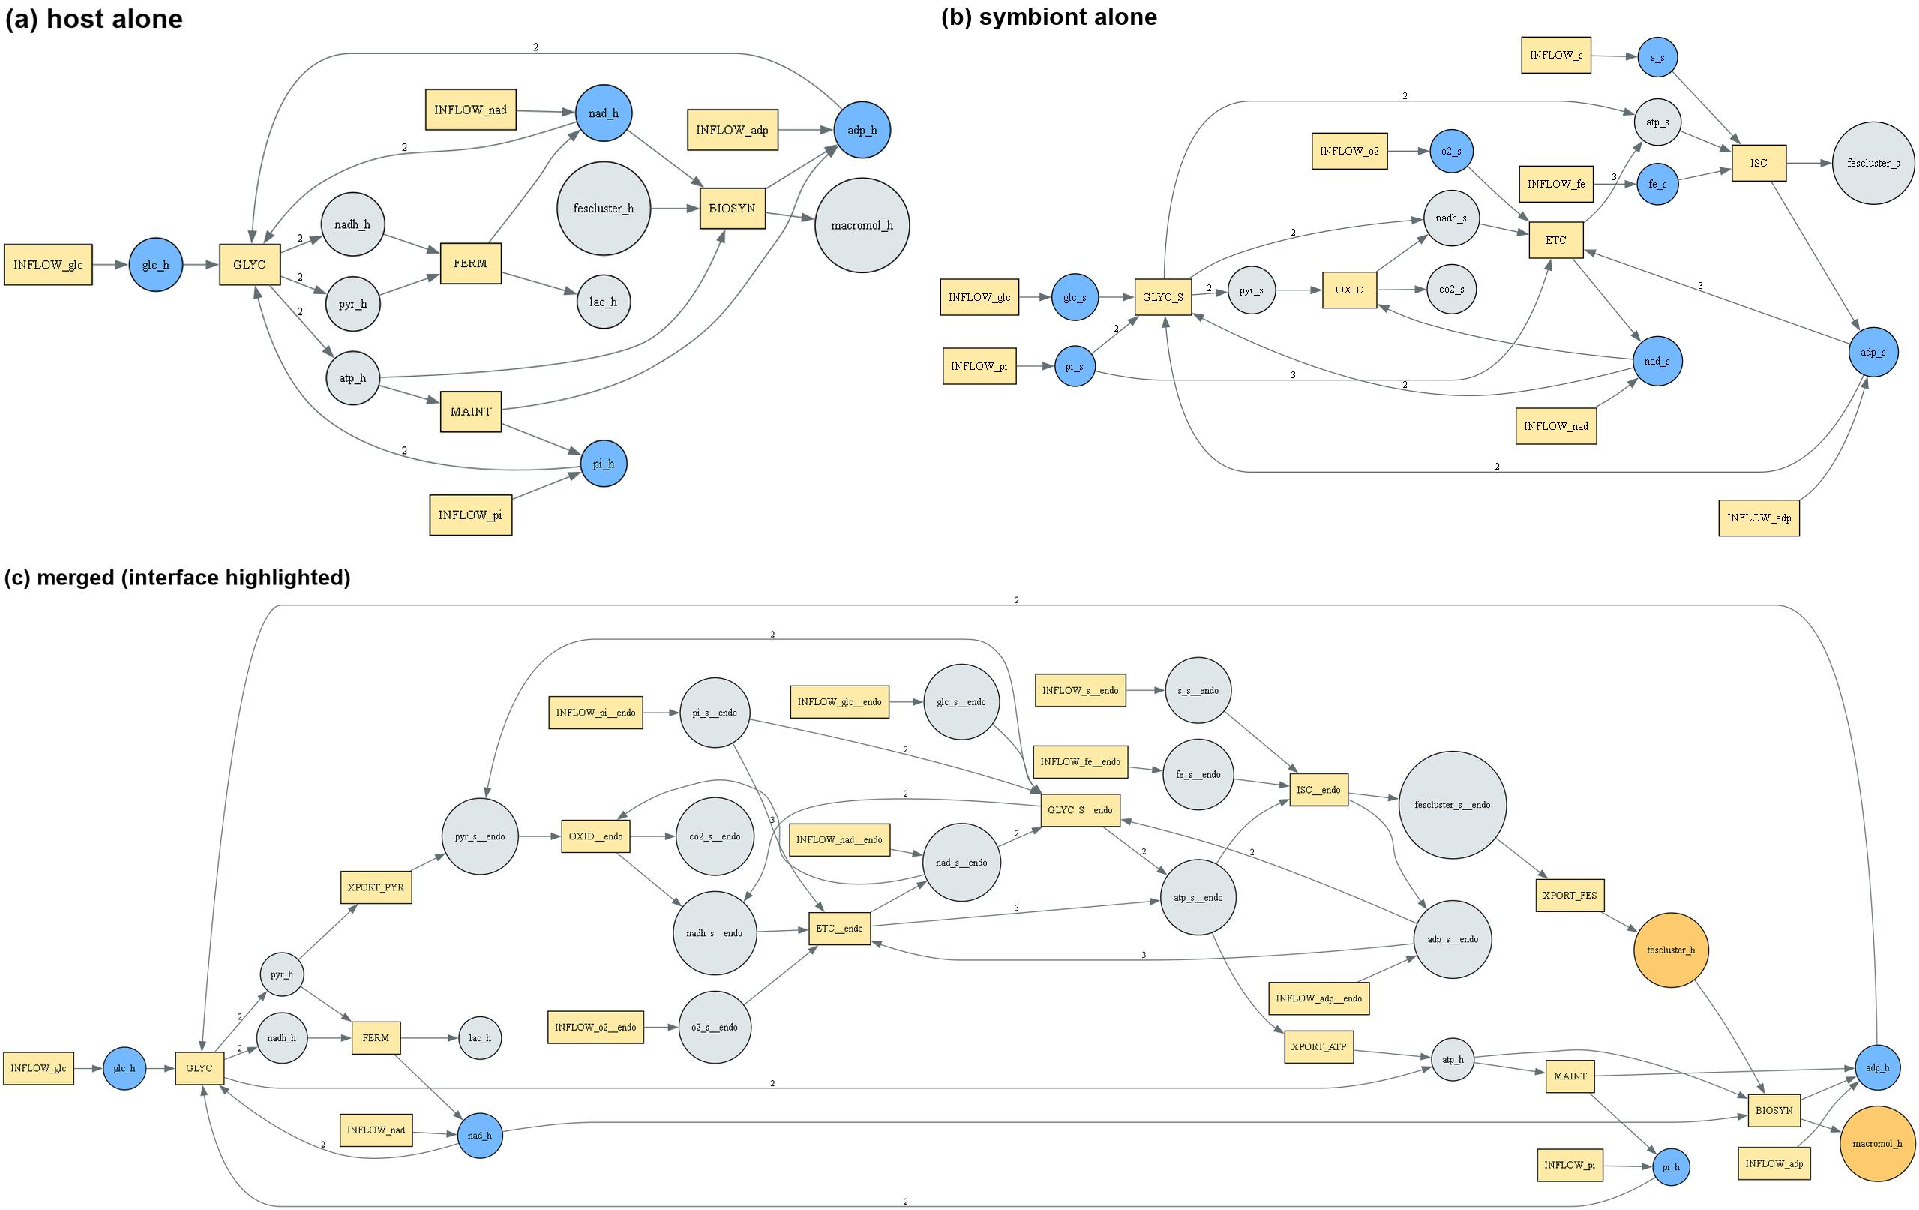
\includegraphics[width=\textwidth]{../figures/fig_native_networks_composite.pdf}
\caption{Toy endosymbiosis model, rendered with pyCOT's native reaction-network visualizer (bipartite species/reaction graph via \texttt{rn\_visualize.py}). \textbf{(a)} Host alone (glycolysis + fermentation). \textbf{(b)} Symbiont alone (glycolysis + oxidative phosphorylation + Fe--S cluster biogenesis). \textbf{(c)} Merged network; the three curated interface reactions (\texttt{XPORT\_PYR}, \texttt{XPORT\_ATP}, \texttt{XPORT\_FES}) connect the two halves, and the two species reachable only once merged (orange) are exactly the ones the toy model was designed around.}
\label{fig:networks}
\end{figure*}

\subsection*{Fusigenic inflow search recovers real biology}
An exhaustive search on the toy host alone -- with no knowledge of the symbiont -- independently rediscovers the exact designed dependency: the Fe--S cluster is the only candidate with nonzero fusion score. On \textit{E.\ coli} core metabolism, an exhaustive sweep over all 65 non-food species instead finds that the top fusigenic candidates are lower-glycolysis and TCA-cycle \emph{intermediates} (2-phosphoglycerate, 3-phosphoglycerate, phosphoenolpyruvate; $\Delta$mean~$=+8.2$), not cofactors -- because the core reconstruction barely represents cofactor biosynthesis at all. A targeted sweep on the larger iAF1260 reconstruction, restricted to the trace metals implicated in the companion paper, recovers that finding directly: molybdate and tungstate each individually produce a real, modest fusion effect ($\Delta$mean~$=+2.0$), consistent with the companion paper's full-medium result (mean size $25.7\to63.7$) being the sum of several individually modest cofactor contributions rather than one dominant one. Fusigenic mechanism is therefore reconstruction-detail-dependent, not fixed (Fig.~\ref{fig:fusigenic}).

\begin{figure*}[t]
\centering
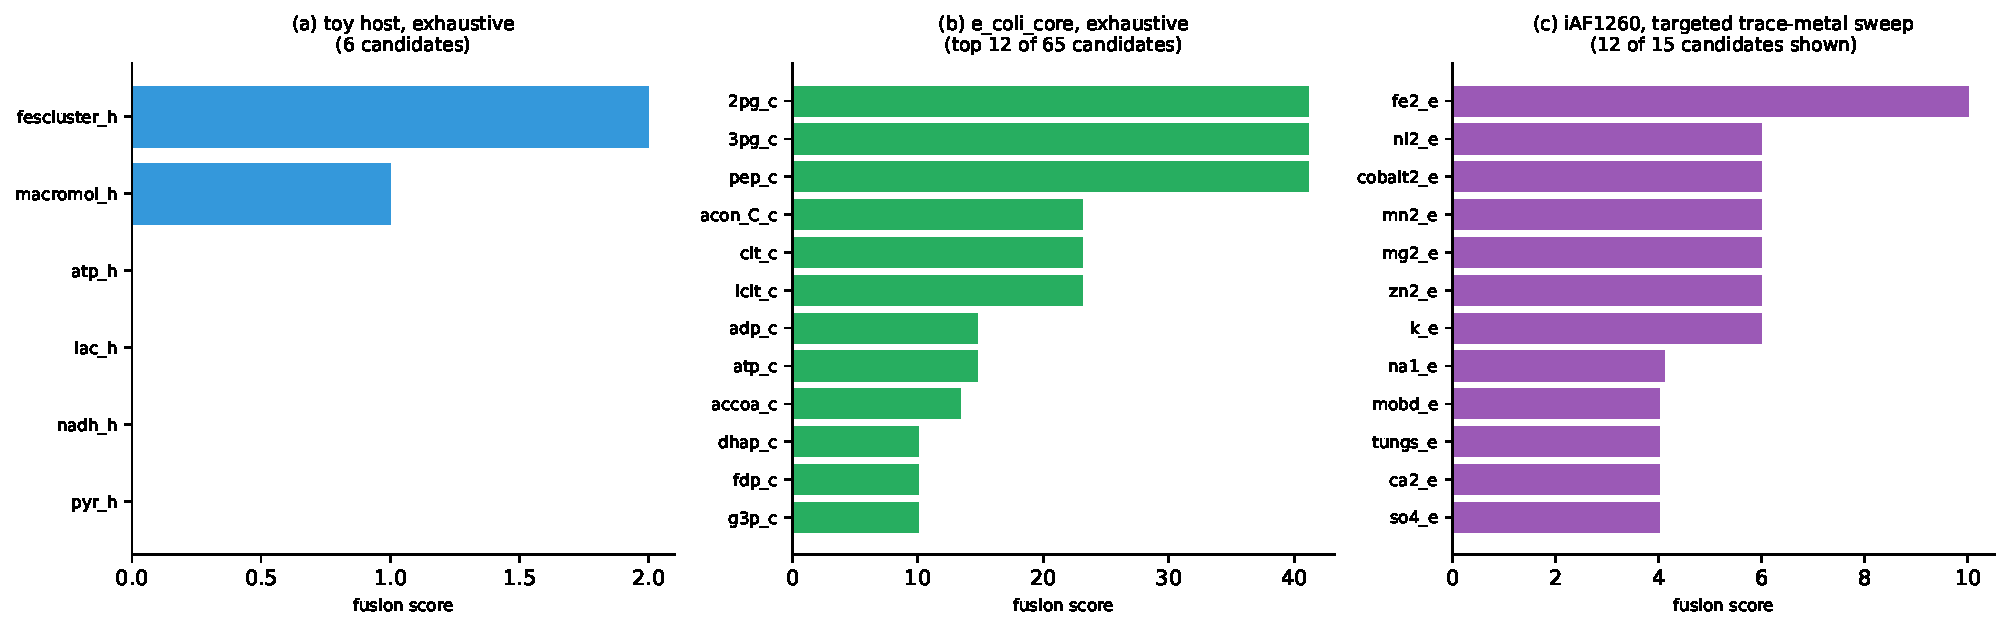
\includegraphics[width=0.85\textwidth]{../figures/fig_fusigenic_search.pdf}
\caption{Fusigenic-inflow search results, ranked by fusion score. \textbf{(a)} Toy host, exhaustive (6 candidates): only the designed Fe--S cluster dependency scores above zero. \textbf{(b)} \textit{E.\,coli} core, exhaustive (top 12 of 65): pathway-intermediate shortcuts dominate. \textbf{(c)} iAF1260, targeted trace-metal sweep: molybdate and tungstate -- the cofactors implicated in the companion paper's full-medium result -- each score individually.}
\label{fig:fusigenic}
\end{figure*}

\subsection*{Real endosymbiotic mergers}
We built two independent real cases using the same generic tooling (Materials and Methods; Table~\ref{tab:cases}).

\textbf{Mitochondrial-type.} Host: \textit{E.\ coli} core metabolism with its three named oxidative-phosphorylation reactions deleted (ATP synthase, cytochrome oxidase, NADH dehydrogenase) -- a fermentative lineage built by deletion from a real curated model. Symbiont: the unmodified reconstruction, standing in structurally for a free-living aerobic respirer. Interface: two reactions, pyruvate in and ATP out. Host and symbiont alone each give 15 ESOs (mean size 15.1, matching the companion paper's own published figures exactly), of which only 5 and 6 respectively (33\%, 40\%) are EOs. Merged: 27 ESOs, mean size 28.2 -- \textbf{100\% hybrid} -- of which 9 (33\%) are EOs. Notably the food closure does \emph{not} grow here (26 vs.\ 26 species): this is \emph{re-integration} of an already-reachable chemistry into fewer, larger, mutually dependent modules, not capability-gain; that only a third of the hybrid ESOs are also EOs shows re-integration at the closure level does not by itself guarantee re-integration at the self-maintaining level.

\textbf{Chloroplast-type.} Host: \textit{Saccharomyces cerevisiae} (iND750), a real heterotrophic eukaryote. Symbiont: \textit{Synechocystis} sp.\ PCC 6803 (iJN678), a real cyanobacterium -- the first genuinely cross-organism test of the relabeling machinery. Interface: the real chloroplast triose-phosphate translocator route (fixed carbon leaves as glyceraldehyde-3-phosphate, the canonical substrate, not free glucose) plus CO\textsubscript{2} recycling back. Host alone: 152 ESOs (mean 42.9, 83 EOs, 55\%); symbiont alone (no light): 63 ESOs (mean 24.0, 13 EOs, 21\%) -- both matching our companion cross-organism comparison exactly at the ESO level. Merged: 221 ESOs, mean size 66.0, \textbf{100\% hybrid}, of which 94 (43\%) are EOs. Here the signature differs again: mean size is almost exactly additive ($42.9+24.0=66.9\approx66.0$) and ESO count \emph{rises} slightly (215$\to$221) rather than falling -- not fusion by the strict count-based definition, but still complete hybridization with a large absolute size jump (max 50$\to$75). Supplying light in addition gives a modest further boost (max~78, 95 EOs, 43\%), as expected since the symbiont already has glucose as carbon source in both variants.

\begin{table*}[t]
\centering
\caption{ESO count (mean size) and, in brackets, the EO sub-count (\% of that ESO count that is LP-verified self-maintaining), host alone / symbiont alone / merged, across all cases. Every merged network is 100\% hybrid at the ESO level.}
\label{tab:cases}
\small
\begin{tabular}{lccc}
\toprule
Case & Host & Symbiont & Merged \\
\midrule
Toy model & 1 (8.0) [1, 100\%] & 1 (12.0) [1, 100\%] & 1 (22.0) [1, 100\%] \\
Mitochondrial-type & 15 (15.1) [5, 33\%] & 15 (15.1) [6, 40\%] & 27 (28.2) [9, 33\%] \\
Chloroplast-type, dark & 152 (42.9) [83, 55\%] & 63 (24.0) [13, 21\%] & 221 (66.0) [94, 43\%] \\
Chloroplast-type, +light & 152 (42.9) [83, 55\%] & 63 (27.0) [14, 22\%] & 221 (69.0) [95, 43\%] \\
\bottomrule
\end{tabular}
\end{table*}

\subsection*{Interface-fragility analysis}
Removing one interface reaction at a time and recomputing ESOs identifies which cross-feeding link is actually necessary (Table~\ref{tab:knockout}). In the toy model, only the Fe--S cluster transporter is load-bearing; removing pyruvate or ATP transport individually changes nothing, because both partners already produce these internally -- the interface adds no new \emph{reachability} there, only, in reality, quantity or efficiency, which a set-based framework does not represent. In the real mitochondrial-type case, knocking out either the pyruvate or the ATP transporter alone gives an \emph{identical} result (28 hybrid ESOs, mean 28.2) -- the real network's own internal redundancy (multiple real routes connect these pools) makes the two transporters redundant with each other. In the chloroplast-type case the two interface reactions are not symmetric: removing carbon export has no measurable effect, but removing CO\textsubscript{2} recycling shrinks both hybrid count (221$\to$214) and mean size (66.0$\to$63.9). Overall, only 1 of 7 interface reactions tested across all three cases was individually load-bearing -- the toy model's Fe--S cluster dependency, which has no redundant alternative route.

\begin{table}[t]
\centering
\caption{Interface-knockout results: hybrid ESO count and mean size with each interface reaction individually removed, vs.\ the full interface. Bold: the one load-bearing reaction found.}
\label{tab:knockout}
\small
\begin{tabular}{llcc}
\toprule
Case & Removed & Hybrid ESOs & Mean size \\
\midrule
Toy & \textit{(none, full)} & 1 & 22.0 \\
Toy & XPORT\_PYR & 1 & 22.0 \\
Toy & XPORT\_ATP & 1 & 22.0 \\
Toy & \textbf{XPORT\_FES} & \textbf{1} & \textbf{20.0} \\
Mito. & \textit{(none, full)} & 27 & 28.2 \\
Mito. & XPORT\_PYR & 28 & 28.2 \\
Mito. & XPORT\_ATP & 28 & 28.2 \\
Chloro. & \textit{(none, full)} & 221 & 66.0 \\
Chloro. & XPORT\_G3P & 221 & 66.0 \\
Chloro. & \textbf{XPORT\_CO2} & \textbf{214} & \textbf{63.9} \\
\bottomrule
\end{tabular}
\end{table}

\begin{figure*}[t]
\centering
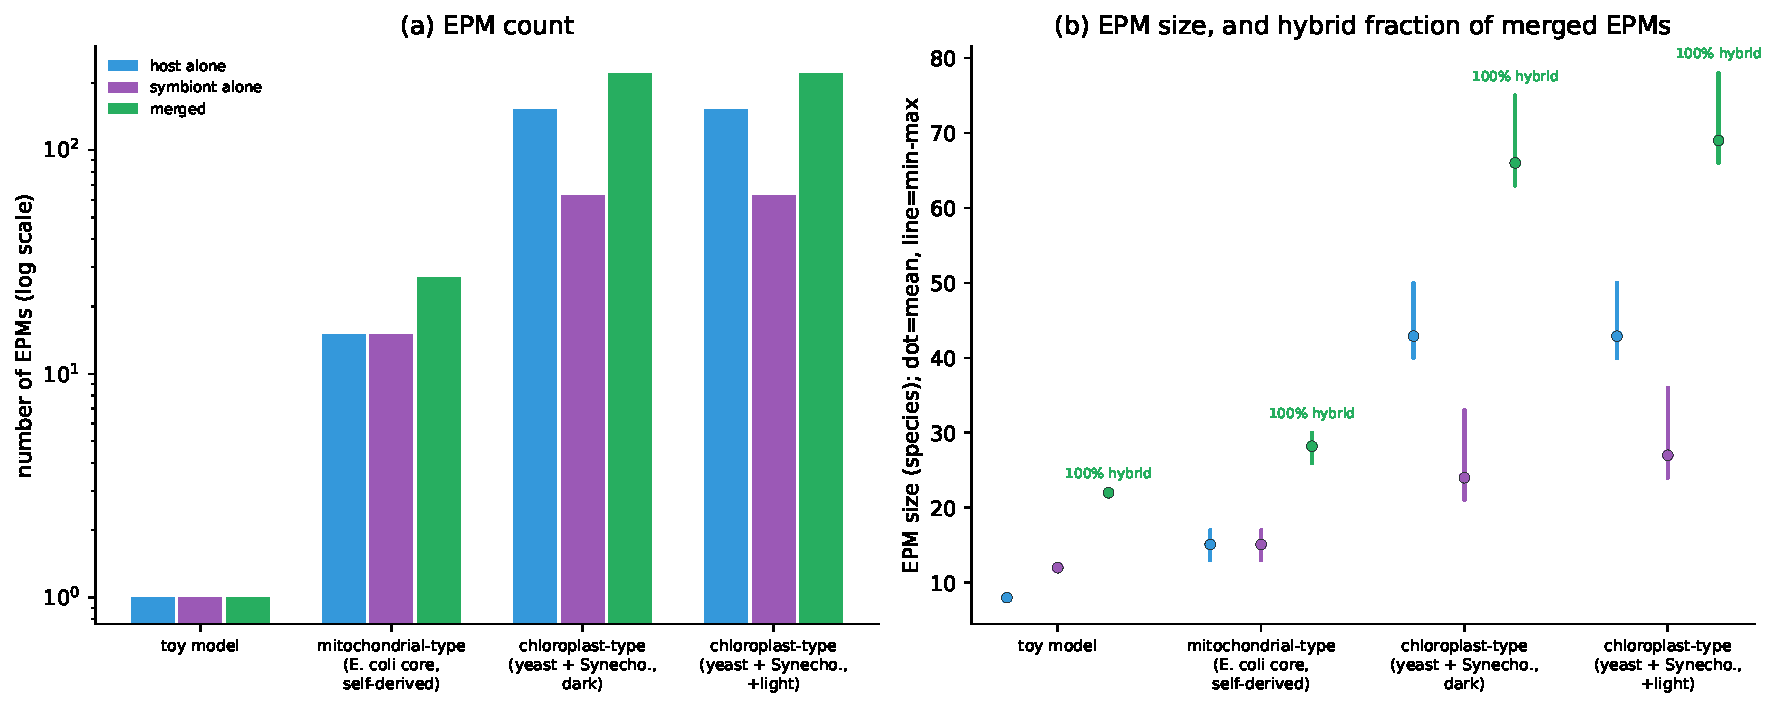
\includegraphics[width=0.68\textwidth]{../figures/fig_complexification_summary.pdf}
\caption{ESO count (a, log scale) and size range (b, min--max with mean; green labels mark 100\% hybrid) for host alone, symbiont alone, and merged, across all four cases. Every merged network is fully hybridized; the count/size pattern (fusion vs.\ additive) differs by case, reflecting the two mechanisms in the text.}
\label{fig:summary}
\end{figure*}

\subsection*{Two mechanisms of complexification}
The cases cluster into two distinct, real mechanisms, both producing the 100\%-hybrid signature but differing in \emph{how}. \emph{Capability-gain} (toy model): the food closure itself grows; new species become reachable only jointly -- the sharpest signature, a literal new capability neither parent has alone. \emph{Re-integration} (mitochondrial-type): the food closure is unchanged, but the same reachable chemistry reorganizes into far fewer, far larger, mutually dependent modules. The chloroplast-type case shows a third, additive/proliferative pattern -- large absolute size growth without count reduction -- plausibly reflecting the far greater combinatorial richness of two large, independently curated genome-scale networks relative to a small or self-derived pair. All three share full hybridization as the mechanism-independent marker of genuine integration.

Closure-level hybridization is not, however, the whole story: across both real mergers the EO fraction of hybrid ESOs settles in a comparable 33--43\% range (mitochondrial-type 33\%; chloroplast-type 43\% in both variants) despite the two cases showing qualitatively different closure-level mechanisms (re-integration vs.\ additive/proliferative) -- suggesting the ESO$\to$EO attrition rate is a comparatively stable property of real merged metabolic networks, largely independent of which closure-level mechanism produced the hybrid ESOs in the first place. Only the toy model, by construction the least combinatorially redundant case, reaches 100\% EO. This mirrors, at the merged-network level, exactly the pattern the companion \textit{E.\,coli} reconstruction-comparison paper reports at the single-network level \cite{velozecoli2026}: most ESOs are not EOs, and the gap widens, not narrows, with network richness.

\subsection*{Hybrid ESOs conserve the host's elementary structure and, when they diverge, diverge on the symbiont's side}
Hybridization says a species set draws from both partners; it does not say whether the module itself is new. For each hybrid ESO of a merged network we split it into a host part and a symbiont part (stripping the interface tag) and ask whether each part is literally identical to some standalone ESO of the corresponding network alone (\matmethods{}). Three outcomes are possible: \emph{conserved} (both parts are already elementary on their own; the interface only glued two pre-existing modules together), \emph{symbiont-emergent} (the host part is conserved but the symbiont part is not, i.e.\ reorganized or extended by the merger), or \emph{host-emergent} (the reverse).

Across every real case tested, the host's own elementary structure is never disturbed: 100\% of hybrid-ESO host parts match a host-alone ESO exactly (Table~\ref{tab:lineage}). What differs between cases is the symbiont side. In the mitochondrial-type merger, all 27 hybrid ESOs are fully \emph{conserved} -- re-integration happens purely by pairing pre-existing host and symbiont modules, changing neither party's own achievable structure. In both chloroplast-type variants, 69/221 (31\%) hybrid ESOs are \emph{symbiont-emergent}: the host part is always an exact match, while the symbiont part is close to, but not identical to (Jaccard 0.82--0.94), a standalone symbiont ESO -- typically a handful of additional species reachable only jointly. No host-emergent or fully-emergent hybrid ESO occurs in any real case; the toy model's single hybrid ESO is the sole host-emergent instance found, consistent with its capability-gain mechanism, where the food closure itself, not just the symbiont's contribution, grows.

Emergent hybridization is also markedly less often self-maintaining: EO fraction is 55\% among conserved hybrid ESOs but only 16--17\% among symbiont-emergent ones in the chloroplast-type cases (the entirely-conserved mitochondrial-type case sits at 33\% overall). Structural novelty at the elementary level and verified self-maintenance move in opposite directions here: the joint modules that require genuine reorganization to exist are also the ones least likely to already carry the flux needed to sustain themselves -- they remain ESOs that would need a still richer environment before qualifying as EOs, not organizations yet.

\begin{table}[t]
\centering
\caption{ESO lineage classification of every hybrid ESO in each merged network: conserved = both host and symbiont parts exactly match a pre-existing standalone ESO; emergent = one part does not (\matmethods{}).}
\label{tab:lineage}
\small
\begin{tabular}{lrrr}
\toprule
Case & Conserved & Symb.-emergent & Host-emergent \\
\midrule
Toy & 0 & 0 & 1 (100\%) \\
Mitochondrial-type & 27 (100\%) & 0 & 0 \\
Chloroplast-type, dark & 152 (69\%) & 69 (31\%) & 0 \\
Chloroplast-type, +light & 152 (69\%) & 69 (31\%) & 0 \\
\bottomrule
\end{tabular}
\end{table}

\section*{Discussion}
The framework developed here is deliberately the structural complement of our own earlier kinetic endosymbiosis model \cite{velozflores2020soft,velozflores2021}: that work represents \emph{how} regulation happens (threshold-gated, bidirectional kinetic control of proliferation and biochemical traffic, calibrated against the coral--\textit{Symbiodinium} system), while the present one asks a prior structural question -- \emph{which} elementary modules become mutually dependent once any interface exists at all, independent of rate constants. A natural and direct next step is to combine them: make interface reactions here conditional in exactly the way our earlier model's host-release and inhibition factors were, gating cross-feeding on a threshold signal rather than leaving it always-on, and asking whether the ESO-level hybridization signature reported here is robust to that regulation being switched off under stress -- which is precisely the dysfunction/bleaching phase of the coral system \cite{velozflores2021}.

The interface-fragility results connect directly to real evolutionary genomics. If a specific cross-fed metabolite has no redundant alternative route -- as in the toy model, but not in either real case tested here -- our framework predicts the corresponding transporter and its regulatory machinery should be under the strongest pressure for retention (or functional transfer to the host genome) during endosymbiont genome reduction, while redundant interface reactions should be more tolerant of loss. That two of the three real interface reactions tested here turned out to be individually dispensable is itself informative, not a null result: it suggests real, richly connected metabolic networks buffer single-transporter loss far more than a minimal, deliberately irreplaceable dependency does, sharpening the prediction from ``interface genes are conserved'' to ``conservation should track computed irreplaceability.''

This is a steady-state, structural framework: it makes no claim about population genetics, fitness, or the dynamics of how a symbiosis is established or fixed, and the interface itself is a curated, explicitly justified modeling choice, not a derived fact. \textit{E.\ coli} core metabolism stands in structurally for ``a free-living aerobic respirer,'' not literally for an alphaproteobacterium; BiGG reconstructions are modern free-living relatives, not the actual ancestral lineages. Within that scope, the central empirical result -- complete ESO hybridization, reproduced independently on a hand-verified toy model and two real, differently constructed genome-scale mergers -- is a specific, checkable structural signature of endosymbiotic integration that required no kinetic parameters to compute. The lineage asymmetry found on top of it -- the host's own elementary structure is never disturbed by the merger, while any reorganization is confined to the symbiont's contribution -- is, again, a purely structural, steady-state observation, not a claim about the population-genetic process of endosymbiont genome reduction; but it is a suggestive structural echo of that real, well-documented asymmetry (endosymbiont genomes shrink and specialize far more than host genomes do), obtained here from network topology alone, before any appeal to selection or drift.

A structurally adjacent literature asks a related minimal-building-block question from a different axiomatic starting point: reflexively autocatalytic, food-generated (RAF) sets decompose into \emph{irreducible} RAFs (irrRAFs), the smallest autocatalytic building blocks a self-sustaining set can be built from, starting from catalysis rather than closure \cite{steel2013minimal}. ESOs and irrRAFs are, informally, analogous objects; whether an irrRAF-decomposition and an ESO/fundamental-synergy decomposition of the same merged network agree, and where they diverge, is a natural, currently open bridge between these two literatures, and could in principle transfer either RAF theory's polynomial-time irrRAF bounds into COT, or the generative ESO construction demonstrated here into RAF enumeration at genome scale.

\matmethods{
All networks use the simple text reaction-network format read by \texttt{pyCOT.io.functions.read\_txt}. ESOs are computed via the ERC$\to$hierarchy$\to$fundamental-synergy/complementarity$\to$ESO pipeline of \texttt{pyCOT.analysis.organizations} \cite{velozbassi}; ESO size of a species mask $m$ is $|m \cup E_0|$ where $E_0$ is the food closure.

\textit{Fusigenic search.} For baseline food $F$ and each candidate $c$, ESOs are recomputed under $F \cup \{c\}$ and compared to baseline; fusion score is $\Delta\text{mean size} \cdot (1+\max(0,-\Delta\text{count}))$ when $\Delta\text{count}\le0$ and $\Delta\text{mean size}>0$, else 0. Exhaustive sweeps are tractable at \textit{E.\,coli} core scale (${\sim}1$--2\,s/candidate); at iAF1260 scale (${\sim}$1500 ERCs, ${\sim}$50--90\,s/candidate) we used a curated trace-metal candidate list rather than the ${\sim}$1400-species exhaustive default.

\textit{ESO$\to$EO verification.} Every ESO is additionally checked for self-maintenance by linear programming (an elementary organization, EO, in the sense of \citet{centler2008computing}'s general organization concept, verified here on ERC-combination closures directly rather than by \citeauthor{centler2008computing}'s species-addition search): given a candidate species set $m$, we build the corresponding sub-stoichiometry matrix $S$ and solve for a flux vector $v$ with $v\ge\epsilon>0$ on every reaction triggered by $m$, $S v \ge -\text{margin}$ (no net depletion of any species in $m$), via \texttt{scipy.optimize.linprog} (\texttt{method=`highs'}). This check is cheap even at genome scale ($<$0.1\,s/ESO; ${\sim}$0.05\,s/ESO on iAF1260-scale mergers) because it is applied to an already-enumerated, elementary/order-0 ESO list rather than to the much larger search space full organization enumeration (with free-species and latent-join completion) would require.

\textit{ESO lineage classification.} For each hybrid ESO of a merged network, species carrying the interface tag are stripped of it and separated from untagged (host) species, giving a host part $H$ and a symbiont part $S$. $H$ is compared by exact set equality against every host-alone ESO, and $S$ (tag-stripped) against every symbiont-alone ESO; a hybrid ESO is \emph{conserved} if both match, \emph{symbiont-emergent}/\emph{host-emergent} if only one does, and \emph{fully-emergent} if neither does. For non-matches we additionally report the closest standalone ESO by Jaccard similarity as a near-miss diagnostic, not a match.

\textit{Endosymbiotic merger.} Every symbiont species and reaction name is relabeled with a tag (\texttt{\_\_endo}) before textual concatenation with the host file; interface reactions are then added explicitly using the relabeled names. An ESO of the merged network is hybrid if its species set intersects both the host's own namespace and the relabeled symbiont namespace.

\textit{Real networks.} \textit{E.\,coli} core, iAF1260, iND750 (\textit{S.\,cerevisiae}), and iJN678 (\textit{Synechocystis} sp.\ PCC 6803) are BiGG genome-scale reconstructions \cite{king2016bigg,orth2010core}, converted to \texttt{pyCOT} format; all use the shared 7-species aerobic core food set (\texttt{co2\_e, glc\_\_D\_e, h2o\_e, h\_e, nh4\_e, o2\_e, pi\_e}) unless noted.

\textit{Network figures.} Fig.~\ref{fig:networks} is rendered directly by pyCOT's native visualizer (\texttt{src/pyCOT/visualization/rn\_visualize.py}: \texttt{create\_bipartite\_graph\_from\_rn}), using \texttt{graphviz} with a left-to-right layout for print legibility; the underlying bipartite graph construction from the real \texttt{ReactionNetwork} object is unmodified.

\textit{Availability.} All code, network files, raw logs, and figures are openly available in the \texttt{pyCOT} repository (\texttt{projects/COT\_Endosymbiosis/}); every number reported here is either copied directly from a logged pipeline run or computed by a script in that directory.
}

\showmatmethods{}

\acknow{This work was supported by the John Templeton Foundation.}

\showacknow{}

\bibliography{bibliography}

\end{document}
